\documentclass[11pt]{amsart}
\usepackage[margin=1.1in]{geometry}
\usepackage{lmodern}
\usepackage[T1]{fontenc}
\usepackage[utf8]{inputenc}
\usepackage{amsmath,amssymb,amsthm}
\usepackage{stmaryrd}
\usepackage{graphicx}
\usepackage{xcolor}
\usepackage{booktabs}
\usepackage{array}
\usepackage{caption}
\captionsetup{font=small}
\captionsetup[lstlisting]{justification=raggedright,singlelinecheck=true}
\usepackage{algorithm}
\usepackage{algpseudocode}
\usepackage{listings}
\usepackage{isabelle-listings}
\usepackage[hidelinks]{hyperref}
\usepackage{xurl}
\usepackage[capitalise,nameinlink]{cleveref}

\definecolor{backcolour}{rgb}{0.96,0.96,0.95}
\lstdefinestyle{isa}{language=Isabelle, backgroundcolor=\color{backcolour},
  basicstyle=\ttfamily\footnotesize, breaklines=true, breakatwhitespace=true,
  columns=flexible, keepspaces=true, captionpos=b, numbers=none, showstringspaces=false,
  aboveskip=6pt, belowskip=8pt, xleftmargin=2pt, xrightmargin=2pt,
  postbreak=\mbox{\textcolor{gray}{$\hookrightarrow$}\space}, mathescape=false}
\lstset{style=isa}
\crefname{lstlisting}{Listing}{Listings}
\Crefname{lstlisting}{Listing}{Listings}

\theoremstyle{plain}
\newtheorem{theorem}{Theorem}
\newtheorem{lemma}{Lemma}[section]
\newtheorem{proposition}[lemma]{Proposition}
\newtheorem{corollary}[lemma]{Corollary}
\theoremstyle{definition}
\newtheorem{definition}[lemma]{Definition}
\newtheorem{remark}[lemma]{Remark}

\newcommand{\thy}[1]{\texttt{#1}}
\newcommand{\C}{\mathbb{C}}
\newcommand{\R}{\mathbb{R}}
\newcommand{\Z}{\mathbb{Z}}
\newcommand{\ab}{\bar a}
\newcommand{\dist}{d}
\newcommand{\Pk}{\mathrm{Pk}}
\newcommand{\El}{E}
\DeclareMathOperator*{\argmax}{arg\,max}
\DeclareMathOperator*{\argmin}{arg\,min}

\begin{document}
\setlength{\emergencystretch}{3em}

\title[Termination of a perturbative sidelobe-nulling method]{When does iterative sidelobe nulling stop?\\
Termination of a perturbative beamforming method,\\ with a mechanized proof in Isabelle/HOL}
\author{Dustin Bryant}
\address{Independent researcher, USA}
\email{brydustin@gmail.com}
\date{November 5, 2026}

\begin{abstract}
The perturbative method shapes the radiation pattern of a phased array by repeatedly placing a
null on its loudest sidelobe.  Starting from the weights that steer the beam to a focus
direction, each iteration evaluates the pattern on a grid of directions, finds its strict local
maxima, sets the main lobe aside, and subtracts from the weight vector the smallest perturbation
that cancels the pattern at the loudest remaining peak above $-20$~dB.  The loop stops when no
such peak remains.  Whether it stops is not obvious: a null in one direction changes the pattern
in every other direction.  We show that the answer depends on the array.  For two nine-element
arrays, a ``double cross'' and a regular octagon, the method stops after at most 20 and at most 10
corrections, for every focus angle and every rule for breaking ties, with a $30^\circ$ guard band or
without one.  Stopping does not mean that every sidelobe is below $-20$~dB: the test sees only the
sampled pattern, and in simulation, at isolated focus angles, the method stops with a sidelobe of up
to $-5.2$~dB that the test misses.  For a 32-element
circular array of radius four wavelengths the stopping condition cannot be met at all for
$20^\circ$ and $30^\circ$ bands.  We also prove a total-correctness Hoare triple for the method
written as a program.  All results are proved in Isabelle/HOL.  The termination proof follows the
pattern of Tucker's computer-assisted proof of the Lorenz attractor: an exact algebraic reduction
to finitely many statements about explicit functions on small intervals, which are then settled by
interval arithmetic with adaptive subdivision.  The difference is that the interval checker is a
function defined and proved sound inside the proof assistant.  We give the main proofs twice: in
ordinary mathematical prose, and as the Isabelle text that was checked.
\end{abstract}

\maketitle

\section{Introduction}\label{sec:intro}

A phased array steers a beam electronically: given the positions of its elements and a desired
focus direction, one chooses complex weights so that the far-field pattern of the array has its
maximum in that direction~\cite{Balanis2016}.  The pattern also has secondary maxima,
\emph{sidelobes}, which waste power and leak signal in unintended directions.  One simple family
of methods reduces them by perturbation~\cite{Steyskal1982,Gong2024,MosierTODO}: starting from the
steering weights, find the loudest sidelobe and subtract from the weight vector the smallest
perturbation that puts a null there; repeat.  The variant studied here, used in the University of
Houston drone-array project, evaluates the pattern on a grid of 1000 directions and stops when
every strict local maximum of these 1000 samples outside a guard band around the focus, other than
the main lobe, is at least 20~dB below the largest sample.

There is no evident reason why this loop should stop.  A null placed in one direction changes
the pattern in every other direction: it can push other sidelobes above the threshold, and it
lowers the main lobe as well, so the threshold, which is relative to the current maximum, moves.
Implementations therefore cap the number of iterations.  We ask whether the cap is ever needed:
for a given array, does the loop stop on its own for every focus direction, and after how many
corrections?

\paragraph{Results.}  The answer depends on the array (\cref{tab:arrays}, \cref{fig:layouts}).

\begin{itemize}
\item \textbf{\Cref{thm:dc}.}  For the nine-element \emph{double cross}, the method stops after at
most 20 corrections, for every real focus angle, with a $30^\circ$ guard band or without one, and
for every rule for breaking ties.
\item \textbf{\Cref{thm:oct}.}  For the regular \emph{octagon}, eight elements on a circle of radius
48.8~mm around a centre element, the same holds with at most 10 corrections.
\item \textbf{\Cref{thm:circ}.}  For a 32-element uniform circular array of radius $4\lambda$, no
choice of weights meets the condition ``every direction outside a $20^\circ$ (or $30^\circ$) band
is at least 20~dB below the maximum'': some direction outside the band always stays above about
$-15.8$~dB (respectively $-17.8$~dB).  A method that stops only when that condition holds therefore
runs forever on this array.
\item \textbf{\Cref{thm:hoare}.}  The method, written as a while-program, satisfies a
total-correctness Hoare triple: it halts, and on halting every strict peak of the sampled pattern outside
the band, other than the main lobe, is at or below $-20$~dB.  The number of corrections is bounded by any bound $D$ for which the run is known to
stop; for the double cross $D = 20$, and for the octagon $D = 10$.
\end{itemize}

\paragraph{What stopping means.}  The theorems hold for every real focus angle, but the test looks
only at the 1000 samples, and there only at strict peaks.  So they say nothing about the pattern
between samples.  In simulation (\cref{sec:unseen}) the stopped pattern is above $-20$~dB at isolated
focus angles: when the top of a sidelobe falls on two samples of equal value, the test does not see
that sidelobe at all.

\begin{table}[t]
\centering
\small
\begin{tabular}{@{}lc>{\raggedright\arraybackslash}p{4.9cm}l>{\raggedright\arraybackslash}p{3.4cm}@{}}
\toprule
array & elements & geometry & band & result\\
\midrule
double cross & 9 & centre; 4 on the axes at 42.21~mm; 4 on the diagonals at 55.40~mm & $30^\circ$, none & stops within 20 corrections (\cref{thm:dc})\\
octagon & 9 & centre; 8 on a circle of radius 48.80~mm & $30^\circ$, none & stops within 10 corrections (\cref{thm:oct})\\
circular & 32 & equally spaced on a circle of radius 400~mm $=4\lambda$ & $20^\circ$, $30^\circ$ & stopping condition unsatisfiable (\cref{thm:circ})\\
\bottomrule
\end{tabular}
\caption{The arrays and what is proved about them.  The wavelength is $\lambda = 100$~mm (3~GHz).}
\label{tab:arrays}
\end{table}

\begin{figure}[t]
\centering
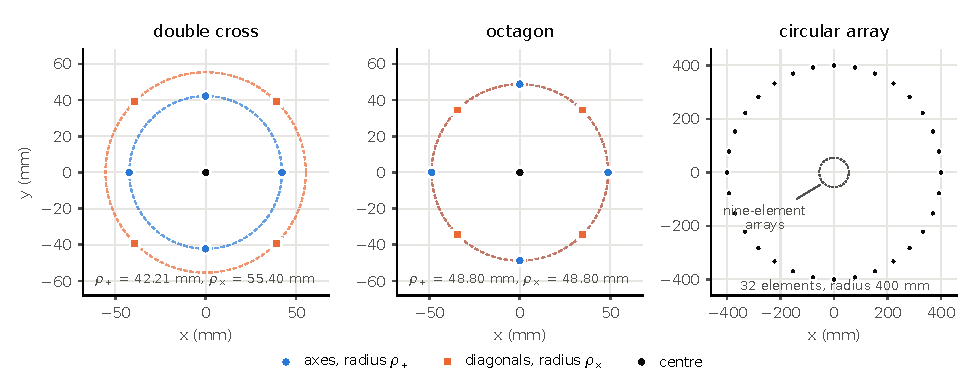
\includegraphics[width=\textwidth]{figs/layouts.pdf}
\caption{Element layouts.  Left: the double cross.  Middle: the regular octagon (\cref{thm:oct}).  Right: the circular array, drawn at a smaller
scale; the dotted circle shows the size of the nine-element arrays.}
\label{fig:layouts}
\end{figure}

\paragraph{Method of proof.}  \Cref{thm:dc} is a statement about uncountably many runs (one for
each focus angle and each tie rule), and each run is a non-smooth process: which sidelobe is
corrected next depends discontinuously on the current pattern.  Our proof follows the pattern of
Tucker's computer-assisted proof that the Lorenz attractor exists~\cite{Tucker1999,Tucker2002}, and
of Hales' proof of the Kepler conjecture~\cite{Hales2005}: an exact argument reduces the theorem to
finitely many explicit inequalities over compact sets, and these are verified with interval
arithmetic and adaptive subdivision~\cite{Moore1966,Tucker2011}.  Here the reduction is algebraic.
After any fixed sequence of corrections the pattern is a fixed linear function of the initial
steering weights (\cref{lem:rows}), so the runs for all focus angles in a small interval can be
followed together, as paths in a finite tree of possible correction sequences.

Unlike the original proofs of Tucker and Hales, our interval checker is not trusted code.  It is
a function defined in higher-order logic and proved sound in Isabelle/HOL~\cite{Paulson1990Next700,NipkowPW02},
and it is then executed by Isabelle's code generator~\cite{HaftmannN10}.  This is the approach of
Immler's verified ODE solver, which formally re-checked the computational part of Tucker's
proof~\cite{Immler18}, and of the verified nonlinear inequalities of the Flyspeck
project~\cite{SolovyevH13,Hales2017}.  \Cref{thm:circ} rests on a certificate from linear
programming whose arithmetic is also checked by Isabelle.  \Cref{thm:hoare} uses the
interaction-tree semantics of Isabelle/UTP~\cite{XiaEtAl2020,FosterHW24,FosterUTP19} and its
verification-condition generator, as in our earlier work on numerical methods~\cite{BryantHF26}.

\paragraph{What is trusted.}  The Isabelle kernel, and, for \cref{thm:dc,thm:oct,thm:circ}, the code
generator and the ML compiler that evaluate the checker.  Isabelle records this dependence: the
oracle set of these theorems is exactly \{\thy{Code\_Generator.holds},
\thy{Code\_Generator.holds\_by\_evaluation}\}.  The general Hoare triple of \cref{sec:hoare} depends
on no oracle.  All results concern exact real arithmetic; \cref{sec:fp} explains how a
floating-point implementation differs.

\paragraph{How to read this paper.}  Each definition and theorem is stated in ordinary notation and
then shown as Isabelle text.  The listings are copied verbatim from the theory files that Isabelle
checked; a reader who does not read Isabelle can skip all of them.
\Cref{sec:method} defines the method, \cref{sec:termination} discusses its stopping condition,
\cref{sec:results} states the results, \cref{sec:proof-dc,sec:proof-circ,sec:hoare} prove them,
and \cref{sec:related,sec:limits} discuss related work and what is not proved.

\section{The method}\label{sec:method}

\subsection{Arrays, patterns and the grid}

An array has $N$ isotropic elements at positions $p_j = (x_j, y_j) \in \R^2$, $j = 0, \dots, N-1$,
and radiates at wavelength $\lambda$; in all our examples $\lambda = 0.1$~m (3~GHz), so the
wavenumber is $k = 2\pi/\lambda = 20\pi$~m$^{-1}$.  In the far field, the response in the azimuth
$\varphi$ to the weights $w \in \C^N$ is the \emph{array factor}
\begin{equation}\label{eq:pattern}
F_w(\varphi) = \sum_{j=0}^{N-1} a_j(\varphi)\, w_j, \qquad
a_j(\varphi) = e^{\mathrm{i} k (x_j \cos\varphi + y_j \sin\varphi)} .
\end{equation}
The vector $a(\varphi)$ is the \emph{steering vector}.  The method looks at $F$ only on the grid
$\varphi_m = 2\pi m/M$, $m \in \Z_M = \{0, \dots, M-1\}$, with $M = 1000$ (spacing $0.36^\circ$),
through the powers $P_w(m) = |F_w(\varphi_m)|^2$.  Grid indices are taken modulo $M$, so $m-1$ and
$m+1$ are the neighbours of $m$ on the circle.

The formal versions (\cref{lst:basics}) use the names \thy{steer}, \thy{patt} and \thy{sq} for
$a$, $F$ and $P$.  An array is a function \thy{p} from element indices to positions together with
its element count \thy{N}; weights are written \thy{c}.  The functions \thy{cis} and \thy{cnj} are
$\theta \mapsto e^{\mathrm{i}\theta}$ and complex conjugation.

\lstinputlisting[caption={The pattern (\thy{Perturbative\_Basics.thy}).}, label=lst:basics]{listings/basics.thy}

\subsection{One correction}

\begin{definition}[correction]
For a grid index $s$, the correction at $s$ is
$C_s(w) = w - \frac{F_w(\varphi_s)}{N}\, \ab(\varphi_s)$, where the bar denotes complex conjugation.
\end{definition}

\begin{lemma}[a correction places a null]\label{lem:null}
$F_{C_s(w)}(\varphi_s) = 0$ for every $w$ and $s$.
\end{lemma}

\begin{proof}
$F_{C_s(w)}(\varphi_s) = F_w(\varphi_s) - \frac{F_w(\varphi_s)}{N}\sum_j a_j(\varphi_s)\ab_j(\varphi_s)
= F_w(\varphi_s) - \frac{F_w(\varphi_s)}{N}\, N = 0$, because $|a_j(\varphi_s)| = 1$.
\end{proof}

\lstinputlisting[caption={\cref{lem:null} in Isabelle (proof omitted).}]{listings/corr_null.thy}

\begin{remark}[the correction is the smallest one]\label{rem:projection}
With the inner product $\langle u, v\rangle = \sum_j u_j \bar v_j$ we have
$F_w(\varphi_s) = \langle w, \ab(\varphi_s)\rangle$ and $\|\ab(\varphi_s)\|^2 = N$, so $C_s$ is the
orthogonal projection of $w$ onto the hyperplane $\{v : F_v(\varphi_s) = 0\}$.  It is therefore the
smallest change of the weights that puts a null at $\varphi_s$, as in the classical null synthesis of
Steyskal~\cite{Steyskal1982}, and
$\|C_s(w)\|^2 = \|w\|^2 - |F_w(\varphi_s)|^2/N$: corrections never increase the norm of the weights.
This remark is not used in the proofs.
\end{remark}

The next lemma is the key to everything that follows: the effect of any fixed sequence of
corrections on the pattern is linear in the weights it started from, with coefficients that do not
depend on those weights.

\begin{lemma}[rows]\label{lem:rows}
Let $g(m,s) = \frac1N \sum_j a_j(\varphi_m)\ab_j(\varphi_s)$.  For a sequence of corrections
$\sigma$ define the \emph{rows} $R^\sigma_{m,j}$ by $R^{()}_{m,j} = a_j(\varphi_m)$ and
$R^{(\sigma,s)}_{m,j} = R^\sigma_{m,j} - g(m,s) R^\sigma_{s,j}$, where $(\sigma, s)$ is $\sigma$
followed by a correction at $s$.  If $C_\sigma$ applies the corrections of $\sigma$ in order, then
\[ F_{C_\sigma(w)}(\varphi_m) = \sum_j R^\sigma_{m,j}\, w_j \qquad\text{for every } w \text{ and } m. \]
\end{lemma}

\begin{proof}
By induction on $\sigma$, using $F_{C_s(v)}(\varphi_m) = F_v(\varphi_m) - g(m,s)\,F_v(\varphi_s)$,
which follows from the definitions by expanding the sum.
\end{proof}

In Isabelle a sequence of corrections is a list with the most recent correction first, and
\thy{exc p N c $\sigma$} applies the corrections $\sigma$ to the weights \thy{c} (\cref{lst:rows}).

\lstinputlisting[caption={Rows and \cref{lem:rows}.}, label=lst:rows]{listings/rows.thy}
\lstinputlisting{listings/rows_lemma.thy}

\subsection{The loop}\label{sec:loop}

The method has the following inputs: the array; a focus angle $t \in \R$; a guard band, given by a
half-width $\Delta \in (0, \pi)$ or absent; and two \emph{tie rules} $\tau_m$ and $\tau_s$, functions
that choose an element from every nonempty finite set of grid indices.  Let
$\dist(\alpha, \beta) = |\alpha - \beta - 2\pi\,\mathrm{round}((\alpha-\beta)/2\pi)| \in [0,\pi]$ be
the distance of two angles on the circle.  For weights $w$ define:

\begin{itemize}
\item the \emph{strict peaks}: $\Pk(w) = \{ m : P_w(m) > P_w(m-1) \text{ and } P_w(m) > P_w(m+1)\}$;
\item the \emph{main lobe}: $m_0(w) = \tau_m\bigl(\argmin_{m \in \Pk(w)} \dist(\varphi_m, t)\bigr)$,
the strict peak nearest to the focus;
\item \emph{outside the band}: $\dist(\varphi_m, t) > \Delta$ (true for every $m$ if there is no band);
\item the \emph{eligible sidelobes}: $\El(w)$, the set of $m \in \Pk(w)$ with $m \neq m_0(w)$,
$P_w(m) > \max_q P_w(q) / 100$, and $m$ outside the band;
\item the \emph{selected sidelobe}: $s(w) = \tau_s\bigl(\argmax_{m \in \El(w)} P_w(m)\bigr)$.
\end{itemize}
The condition $P_w(m) > \max_q P_w(q)/100$ says that the level $10\log_{10}(P_w(m)/\max_q P_w(q))$
is above $-20$~dB.

\begin{algorithm}[t]
\caption{The perturbative method (one beam, one correction per iteration).}\label{alg:method}
\begin{algorithmic}[1]
\State $w \gets \ab(t)$ \Comment{unit amplitudes; the phases steer the beam to $t$}
\While{$\El(w) \neq \emptyset$}
  \State $w \gets C_{s(w)}(w)$ \Comment{null the loudest eligible sidelobe}
\EndWhile
\State \Return $w$
\end{algorithmic}
\end{algorithm}

\Cref{alg:method} is the method.  It has no iteration cap.  Its \emph{run} is the sequence
$w_0 = \ab(t)$ and $w_{n+1} = w_n$ if $\El(w_n) = \emptyset$, $w_{n+1} = C_{s(w_n)}(w_n)$
otherwise.  The run \emph{stops within $D$ corrections} if $\El(w_n) = \emptyset$ for some
$n \le D$.  \Cref{alg:method} is the MATLAB code \thy{perturb\_method\_v25b.m} of the project,
restricted to one beam, no prescribed null and one correction per iteration, with its strict-peak
rule (\thy{findpeaks\_fast}) and in exact arithmetic.  \Cref{fig:run} shows a run.

\begin{figure}[t]
\centering
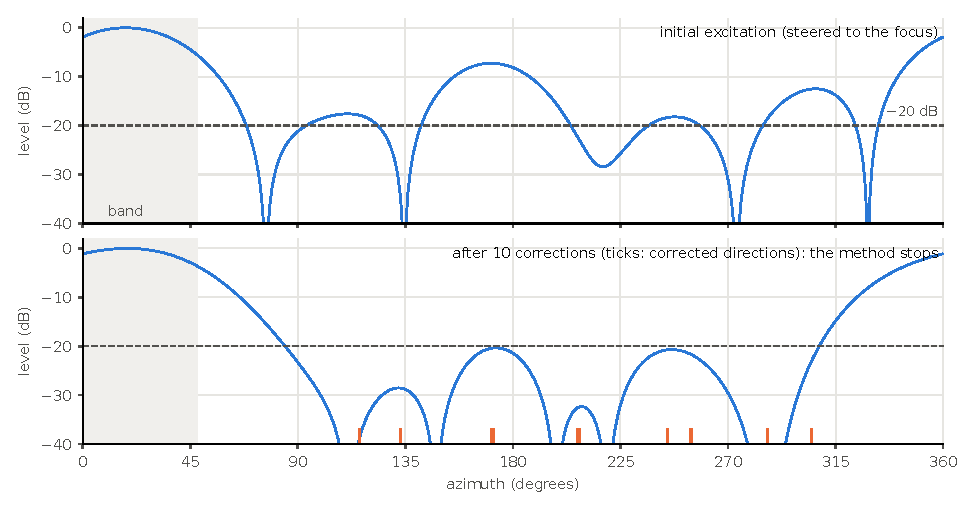
\includegraphics[width=\textwidth]{figs/run_double_cross.pdf}
\caption{A run of \cref{alg:method} for the double cross, focus $17.9^\circ$, guard band
$30^\circ$ (shaded).  Top: the level $10\log_{10}(P_w(m)/\max_q P_w(q))$ of the initial pattern;
the loudest sidelobe outside the band is at $-7.3$~dB.  Bottom: after 10 corrections, at the
directions marked at the bottom, every strict peak outside the band is below $-20$~dB and the method
stops.  (Floating-point simulation; Isabelle's interval evaluation of the same run gives the same
ten corrections.)}
\label{fig:run}
\end{figure}

The formal definitions are in \cref{lst:algorithm}.  Two names need explanation.
\thy{in\_band band t m} means ``$m$ is in the sidelobe region'', that is, outside the guard band;
\thy{band} is \thy{None} for no band and \thy{Some $\Delta$} for the half-width $\Delta$.
\thy{tie\_rule tm ts} says only that each of the two functions picks an element of every nonempty
finite set; nothing else is assumed about them.

\lstinputlisting[caption={The method (\thy{Algorithm.thy}).}, label=lst:algorithm]{listings/algorithm.thy}

\section{The stopping condition}\label{sec:termination}

\subsection{What the stopping test says}

When the loop exits, $\El(w) = \emptyset$, which unfolds to the following.

\begin{lemma}\label{lem:stopped}
If $\El(w) = \emptyset$, then every strict peak $m \neq m_0(w)$ outside the band satisfies
$10\log_{10}(P_w(m)/\max_q P_w(q)) \le -20$.
\end{lemma}

This is the test that the code implements; call it~(I).  The specification that one usually has in
mind is stronger:
\begin{itemize}
\item[(S)] every grid direction outside the band satisfies $P_w(m) \le \max_q P_w(q)/100$.
\end{itemize}
(S) implies (I), but not conversely: (I) looks only at strict peaks.  A sidelobe whose peak lies
inside the band can have a skirt that extends outside the band above $-20$~dB without being a strict
peak there, and (I) does not see it.  \Cref{thm:circ} is about (S); \cref{thm:dc,thm:hoare} are about~(I).

\subsection{The parts of the condition}

Each part of the stopping test matters for whether and how the loop stops.

\emph{The threshold is relative to the current maximum.}  Every correction changes the main lobe as
well as the sidelobes, so the threshold $\max_q P_w(q)/100$ moves from one iteration to the next.

\emph{The guard band.}  The main lobe has a width.  Without a band, every strict peak except the one
nearest the focus counts as a sidelobe, including peaks on the flank of a broad main lobe.

\emph{The grid.}  The test looks at the pattern only at the $M = 1000$ grid directions, and there only
at strict peaks.  The focus is not restricted to the grid: the theorems hold for every real focus
angle.  \Cref{sec:unseen} describes what the test does not see.

\emph{Ties.}  Two peaks can be at the same distance from the focus, or have the same power.  For
symmetric arrays such exact ties occur, for instance when the focus lies on a symmetry axis.  The
code breaks ties by taking the first index, as MATLAB's \texttt{min} and \texttt{sort} do; our
theorems hold for every tie rule, so they cover this rule and any other.

\subsection{Why the loop need not stop}

The norm of the weights decreases at every correction (\cref{rem:projection}), but this does not
force termination, because the stopping test is relative: the pattern can shrink as a whole while
keeping a sidelobe above the threshold.  Two phenomena show that the stopping condition deserves
attention.

\emph{The condition can be unsatisfiable.}  For the circular array, \cref{thm:circ} shows that no
weights at all satisfy (S) for a $20^\circ$ or $30^\circ$ band.

\emph{The loop can stop for a bad reason.}  The test can also be met by destroying the beam.

\begin{proposition}[a degenerate stop]\label{prop:collinear}
Suppose that all elements lie on the $x$-axis, that the focus $t = \varphi_m$ is a grid direction
with $m \notin \{0, M/2\}$ that is a strict peak of the initial pattern, that $\dist(-t, t) > \Delta$,
and that the tie rule selects the mirror index $M - m$ in the first iteration.  Then
$w_1 = 0$, and the run stops after one correction with the zero pattern.
\end{proposition}

\begin{proof}
Since $y_j = 0$, $a_j(-\varphi) = a_j(\varphi)$ for all $\varphi$.  Hence
$P_{w_0}(M-m) = P_{w_0}(m) = |\sum_j a_j(t)\ab_j(t)|^2 = N^2$, the largest possible value, and
$M - m$ is a strict peak because the grid is symmetric under $m \mapsto M - m$.  The main lobe is
$m$ (distance $0$ from the focus), and $M - m$ lies outside the band, so $M - m$ is eligible and
as loud as any peak.  If it is selected, then $w_1 = \ab(t) - \frac{N}{N}\ab(-t) = 0$.  The zero
pattern has no strict peaks, so $\El(w_1) = \emptyset$.
\end{proof}

So ``the method stops'' and ``the method succeeds'' are different statements.  Our theorems are about
the first, together with the sidelobe property of \cref{lem:stopped} at the stop; they say nothing
about the level of the main lobe at the end.  (\Cref{prop:collinear} is not formalized.)

\subsection{What the test does not see}\label{sec:unseen}

Two angles occur in the theorems.  The focus $t$ is arbitrary: \cref{thm:dc,thm:oct} hold for every
real $t$, because each interval of foci in the proof is covered completely (\cref{prop:sound}).  The
look direction $\varphi$ is not: the method evaluates the pattern only at the grid directions
$\varphi_m$, and its test, and hence \cref{lem:stopped}, concerns only those $M$ values and only
their strict peaks.  At the stop, the pattern can be above $-20$~dB in three ways that the test does
not see.

The numbers below come from a floating-point simulation with the $30^\circ$ band (without a band the
runs are the same), at 4{,}501 equally spaced focus angles in $[0, \pi/4]$ and at the focus angles
where the sequence of corrections changes, located by bisection.  At each stop the pattern was
evaluated on a grid 64 times finer.  They are observations, not theorems.

\emph{The main lobe is wider than the band.}  Both arrays are about one wavelength across.  Just
outside the $30^\circ$ band the stopped pattern is between $-4.5$ and $-2.3$~dB for the double cross,
and between $-4.0$ and $-2.7$~dB for the octagon; this is the flank of the main lobe.  So (S) fails at
every stop that we simulated, and for these arrays only the implemented test~(I) can be met.

\emph{Flat tops.}  A sidelobe whose top falls on two adjacent grid points with equal values has no
strict peak, so the test does not see it.  This does happen.  As the focus moves, the top of a
sidelobe moves from one grid point to the next; on the way the difference of the two values changes
sign, and by the intermediate value theorem there is a focus at which it is zero.  If that sidelobe
is the only one still above $-20$~dB, the run stops there without correcting it.  We found 82 such
focus angles for the double cross, where the missed sidelobe is between $-20.0$ and $-5.2$~dB, and 15
for the octagon, between $-19.5$ and $-15.2$~dB.  For the double cross near $t = 0.312^\circ$ the run
stops after no correction at all, with a sidelobe at $-5.2$~dB.  These focus angles are isolated, but
the theorems cover them, and at them the method stops early.

\emph{Between grid points.}  The test compares grid values with the largest grid value.  When a
sidelobe ends exactly at the threshold, its true maximum between two grid points can lie slightly
above $-20$~dB.  For the double cross we found 8 such stops, with an excess of at most $0.0004$~dB;
for the octagon we found none.

None of this affects \cref{thm:dc,thm:oct}, which are about stopping.  It limits what the stop
means.

\subsection{Exact and floating-point arithmetic}\label{sec:fp}

Our theorems concern the method in exact real arithmetic.  A floating-point implementation can also
stop for reasons that have nothing to do with the pattern.  As the weights shrink, the computed
powers eventually underflow, the levels in decibels become $-\infty$ or \texttt{NaN}, and the
comparisons that define $\El(w)$ become false.  In a floating-point simulation of the circular array
of \cref{thm:circ} without a guard band, the implemented code ran for 35{,}414 corrections and then
stopped in this way, with a sidelobe still at about $-3$~dB.  This is an observation, not a theorem.
For the double cross the runs stop after at most 20 corrections, and in our simulations nothing of
this kind happens, but we have not proved a floating-point version of \cref{thm:dc}.

\subsection{The hypotheses of our theorems}

For definiteness, everything we prove is about \cref{alg:method} with: exact arithmetic; the grid
$M = 1000$; the threshold $-20$~dB relative to the current maximum on the grid; strict peaks; the
main lobe defined as the strict peak nearest the focus; one correction per iteration at a loudest
eligible peak; arbitrary tie rules; initial weights $\ab(t)$; and element positions equal to the
binary64 values given in \cref{app:positions}.

\section{Results}\label{sec:results}

\begin{theorem}[the double cross stops]\label{thm:dc}
Let $p$ be the double cross (\cref{app:positions}), $N = 9$.  For every focus angle $t \in \R$, for
the guard band $\Delta = 30^\circ$ and for no band, and for all tie rules $\tau_m$, $\tau_s$, the run
of \cref{alg:method} stops within 20 corrections.
\end{theorem}

\lstinputlisting[caption={\Cref{thm:dc} (\thy{Double\_Cross\_Final.thy}).  \thy{dcp} is the double
cross; $\pi/6 = 30^\circ$.}, label=lst:dc]{listings/dc_final.thy}

The bound 20 is the depth of the deepest branch that the proof explores, over all focus angles and
all tie rules.  For one tie rule (the first index, as in MATLAB) and in floating point, the runs use
at most 16 corrections (\cref{fig:focus}); the bound of the theorem also covers the other tie rules,
whose runs can be longer.

\begin{figure}[t]
\centering
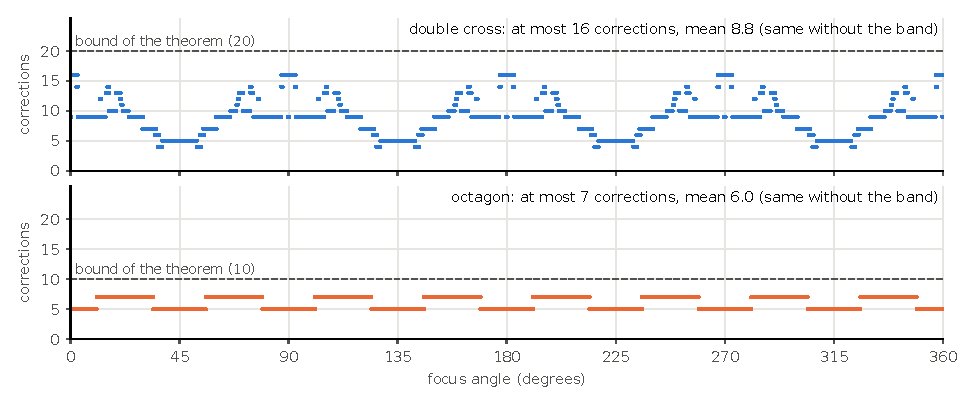
\includegraphics[width=\textwidth]{figs/corrections_vs_focus.pdf}
\caption{Corrections used at 3{,}600 focus angles by the double cross (top) and the octagon
(bottom), for one tie rule (first index) in a floating-point simulation, with the $30^\circ$ band;
without the band the numbers are the same at every angle.  \Cref{thm:dc,thm:oct} bound them by 20 and
10 for every focus angle and every tie rule.}
\label{fig:focus}
\end{figure}

The same holds for a second nine-element array, the regular octagon: a centre element and eight
elements at distance 48.8~mm, at the angles $k\pi/4$.  So that the symmetry argument of
\cref{sec:symmetry} applies exactly, its positions are the binary64 numbers $(\pm a, 0)$,
$(0, \pm a)$ and $(\pm b, \pm b)$, with $a$ the binary64 number nearest 48.8~mm and $b$ the one nearest
$a/\sqrt2$ (\cref{app:positions}); the diagonal elements are then within $10^{-17}$~m of the circle.

\begin{theorem}[the octagon stops]\label{thm:oct}
Let $p$ be the octagon (\cref{app:positions}), $N = 9$.  For every focus angle $t \in \R$, for the
guard band $\Delta = 30^\circ$ and for no band, and for all tie rules $\tau_m$, $\tau_s$, the run of
\cref{alg:method} stops within 10 corrections.
\end{theorem}

\lstinputlisting[caption={\Cref{thm:oct} (\thy{Octagon\_Final.thy}).  \thy{ocp} is the octagon.},
label=lst:oct]{listings/oc_final.thy}

\begin{theorem}[the circular array cannot meet (S)]\label{thm:circ}
Let $p$ consist of 32 elements equally spaced on the circle of radius $0.4$~m $= 4\lambda$, let the
focus be $0$, and let $Q_\Delta = \{ m : \dist(\varphi_m, 0) > \Delta\}$ be the grid directions
outside the band.  For every weight vector $w \in \C^{32}$,
\[ \max_{m \in Q_{20^\circ}} |F_w(\varphi_m)| \ \ge\ 0.1614\, \max_{m} |F_w(\varphi_m)|, \qquad
   \max_{m \in Q_{30^\circ}} |F_w(\varphi_m)| \ \ge\ 0.1286\, \max_{m} |F_w(\varphi_m)| . \]
Consequently, if $w \neq 0$, then (S) fails for both bands: since $20\log_{10} 0.1614 \approx -15.8$
and $20\log_{10} 0.1286 \approx -17.8$, some direction outside the band is above $-20$~dB.
\end{theorem}

\lstinputlisting[caption={\Cref{thm:circ} (\thy{Circular\_Floor.thy}, \thy{Circular\_Result.thy}).
Angles in \thy{Qset} are in degrees; \thy{cv} is an arbitrary weight vector.}, label=lst:circ]{listings/circ_maxq.thy}
\lstinputlisting{listings/circ_result.thy}

\begin{theorem}[total correctness of the program]\label{thm:hoare}
Write \cref{alg:method} as a while-program over the state of \cref{sec:hoare}.  If the run with
focus $t$, band $\Delta$ and tie rules $\tau_m, \tau_s$ stops within $D$ corrections, then the
program halts from every initial state; at the end, $n \le D$, the weights equal $w_n$, and every
strict peak other than the main lobe and outside the band is at or below $-20$~dB.  In particular,
this holds with $D = 20$ for the double cross and with $D = 10$ for the octagon, for every focus, both
bands and all tie rules.
\end{theorem}

The formal statement is in \cref{lst:hoare-main,lst:hoare-dc} of \cref{sec:hoare}.

\section{Proof of \texorpdfstring{\cref{thm:dc}}{Theorem 1}}\label{sec:proof-dc}

\subsection{Strategy}

The proof has four steps.
\begin{enumerate}
\item By the symmetry of the double cross, it is enough to treat focus angles in $[0, \pi/4]$
(\cref{sec:symmetry}).
\item Cover $[0, \pi/4]$ by the 3{,}232 intervals $[j\,2^{-12}, (j+1)\,2^{-12}]$, $j < 3232$; they
reach $3232 \cdot 2^{-12} \approx 0.7891 > \pi/4 \approx 0.7854$.
\item For each interval $T$, a checker explores every sequence of corrections that a run with focus
in $T$ could make, splitting $T$ where necessary.  Success certifies that every run with focus in $T$
stops within 20 corrections, for every tie rule (\cref{sec:tree,sec:enclosures,sec:classify,sec:search}).
\item The checker succeeds on all $2 \times 3232 = 6464$ intervals (one set for each band).  Each
success is a lemma proved inside Isabelle by evaluating the checker (\cref{sec:computation}).
\end{enumerate}

\subsection{Runs as paths in a tree}\label{sec:tree}

Fix a sequence of corrections $\sigma$.  By \cref{lem:rows}, after the corrections $\sigma$ the power
at grid index $m$, as a function of the focus, is
\begin{equation}\label{eq:S}
P_m(t) = S(R^\sigma_m; t), \qquad S(r; t) = \Bigl|\sum_j r_j\, e^{-\mathrm{i}\psi_j(t)}\Bigr|^2, \qquad
\psi_j(t) = k(x_j \cos t + y_j \sin t),
\end{equation}
because the initial weights are $\ab_j(t) = e^{-\mathrm{i}\psi_j(t)}$.  The rows $R^\sigma$ do not depend
on $t$.  Therefore the state of a run is determined by its focus $t$ and by the sequence $\sigma$ of
corrections it has made.  All runs with focus in an interval $T$ are paths in one tree: its nodes
are correction sequences, and the children of $\sigma$ are $(\sigma, s)$ for the indices $s$ that a
run in the state $\sigma$ could correct next.  In Isabelle this is \thy{sq\_exc\_SS} together with
\thy{run\_exc}, which says that the run is the initial weights corrected by the list \thy{corrs} of
the corrections made so far.

\lstinputlisting{listings/sq_rows.thy}
\lstinputlisting{listings/run_exc.thy}

\subsection{Enclosures on an interval of focus angles}\label{sec:enclosures}

On an interval $T = [c - h, c + h]$ we bound $S(r; \cdot)$ by its Taylor expansion at the midpoint.

\begin{lemma}[second-order bound]\label{lem:taylor}
For $r \in \C^N$ let $B = \sum_j |r_j|$, $D = \sum_j |r_j|\gamma_j$ and
$E = \sum_j |r_j|(\gamma_j + \gamma_j^2)$, with $\gamma_j = k\,\|p_j\|$, and let $H = 2(D^2 + BE)$.
Then for all $t, c \in \R$,
\[ |S(r;t) - S(r;c)| \le |S'(r;c)|\,|t - c| + \tfrac{H}{2}(t - c)^2 . \]
\end{lemma}

\begin{proof}
Write $G(t) = \sum_j r_j e^{-\mathrm{i}\psi_j(t)}$, so that $S = |G|^2$ and $S'' = 2|G'|^2 + 2\,\mathrm{Re}(\bar G G'')$.
Since $|\psi_j'| \le \gamma_j$ and $|\psi_j''| \le \gamma_j$, we have $|G| \le B$, $|G'| \le D$ and
$|G''| \le E$, hence $|S''| \le H$.  Taylor's theorem with the Lagrange remainder gives the bound.
\end{proof}

\lstinputlisting[caption={\cref{lem:taylor} (\thy{Taylor\_Enclosure.thy}).  \thy{SS r p N t} is $S(r;t)$,
\thy{SS1} its derivative, \thy{Hc} the constant $H$; \thy{gam p j} is $\gamma_j$.}]{listings/taylor.thy}
\lstinputlisting{listings/hc.thy}

A second bound of the same kind, with constant $H(r) + H(r')$, controls the difference
$S(r;t) - S(r';t)$ of two powers directly.  This is sharper than subtracting two separate
enclosures, and it is what decides the peak tests $P_m > P_{m \pm 1}$.

The checker evaluates $S(r;c)$ and $S'(r;c)$ at the midpoint with interval arithmetic on binary
floating-point numbers with outward rounding and 53-bit precision; cosines and sines are enclosed by
the verified approximations of Isabelle's \thy{Approximation} library~\cite{Holzl2009}.  The rows
themselves are carried along the tree as interval enclosures: every correction updates them by the
recursion of \cref{lem:rows}, evaluated in interval arithmetic.  Lemma~\ref{lem:taylor} then gives,
for every $t \in T$, an interval containing $P_m(t)$, and one containing $P_m(t) - P_{m\pm1}(t)$.

\subsection{Classifying the grid directions at a node}\label{sec:classify}

At a node $(T, \sigma)$ the checker uses these enclosures to classify every grid index $m$, in a way
that is valid for every focus $t \in T$ simultaneously.
\begin{itemize}
\item $m$ is \emph{possibly a peak} (\thy{PP}) if both neighbour differences may be positive, and
\emph{certainly a peak} (\thy{CP}) if both are certainly positive.
\item $m$ is \emph{possibly} or \emph{certainly outside the band} (\thy{PO}, \thy{CO}), from bounds on
$\dist(\varphi_m, t)$ over $T$; the distance is 1-Lipschitz in $t$.
\item $m$ is \emph{excluded} (\thy{EXC}) if it lies in a run of one or two adjacent possible peaks that
is nearer to every focus in $T$ than every other possible peak.  If such a run contains a strict peak,
that peak is the main lobe; since two adjacent grid points cannot both be strict peaks, nothing in the
run can be eligible.
\item The lower bounds give $\mathrm{GL} = \max_m \underline{P_m} \le \max_q P(q)$ and the threshold
$\mathrm{TH} = \mathrm{GL}/100$, rounded downward.  The upper bounds give $\mathrm{US}$, the largest
upper bound $\overline{P_m}$ over the indices that could be eligible (possible peaks, possibly outside
the band, not excluded).
\end{itemize}
The node is \emph{terminal} if $\mathrm{US} \le \mathrm{TH}$.  Then no index is eligible, for any focus
in $T$ (\cref{lst:classify}, \thy{terminal\_sound}).  Otherwise the \emph{candidates} are the indices
that could be eligible and whose upper bound reaches $\mathrm{TH}$, except those whose upper bound is
below $\mathrm{LL}$.  Here $\mathrm{LL}$ is the largest lower bound of an index that is certainly a
strict peak, certainly outside the band and certainly not the main lobe; such an index is louder than
any index whose upper bound is below $\mathrm{LL}$, and eligible whenever that index is, so the latter
cannot be selected.  Every index that some run could select is a candidate
(\thy{sel\_cand}).

\lstinputlisting[caption={Classification of a node and its two soundness lemmas (\thy{Classify.thy}).
\thy{R} and \thy{Hb} are the row enclosures and curvature bounds of the node; \thy{lo}, \thy{hi}
are the ends of $T$.}, label=lst:classify]{listings/classify.thy}
\lstinputlisting{listings/terminal_sound.thy}
\lstinputlisting{listings/sel_cand.thy}

\subsection{The search and its soundness}\label{sec:search}

The search (\cref{lst:verify}) starts at the root $\sigma = ()$ over an interval $T$.  At a node it
first checks the distance bounds (\thy{all\_ok}); if the node is terminal it succeeds.  Otherwise
it computes the candidates.  If $T$ is wider than $w_{\min} = 2^{-26}$, and either the number of
candidates is not exactly one or the depth limit $D_{\max} = 20$ has been reached, it splits $T$ at
its midpoint \thy{tc lo hi} and searches both halves.  If it does not split, it succeeds when there
is no candidate, because a selected index would be a candidate; it fails when the depth limit has
been reached; and otherwise it searches every child $(\sigma, s)$, one for each candidate $s$.  The argument \thy{f} is fuel, a bound on the recursion depth that makes \thy{verify}
a total function.

\lstinputlisting[caption={The search (\thy{Search.thy}).}, label=lst:verify]{listings/verify.thy}

\begin{proposition}[soundness]\label{prop:sound}
If the search succeeds on $[\mathrm{lo}, \mathrm{hi}]$, then for every $t \in [\mathrm{lo}, \mathrm{hi}]$
and all tie rules the run stops within $D_{\max}$ corrections.
\end{proposition}

\begin{proof}
We prove, by induction on the fuel, that success at a node $([\mathrm{lo},\mathrm{hi}], \sigma)$
implies: every run whose focus lies in $[\mathrm{lo},\mathrm{hi}]$ and whose first corrections are
$\sigma$ stops within $D_{\max}$.  At a terminal node the run's state is described by the node
(\cref{sec:tree}), and \thy{terminal\_sound} gives $\El = \emptyset$.  At a split, the focus lies in
one of the halves.  At a branching node, the run either has stopped, or its next correction is a
candidate by \thy{sel\_cand}, and the child for that candidate certifies the rest of the run.  Exact
ties need no special treatment: the candidates include every index that any tie rule could select.
The root has $\sigma = ()$, which every run starts with.
\end{proof}

The executable checker \thy{check\_sector} (\cref{lst:sector}) computes the kernel and the curvature
tables once and runs an implementation of the search on lists; \thy{verify\_impl\_eq} proves it equal
to \thy{verify}.

\lstinputlisting{listings/verify_sound.thy}
\lstinputlisting[caption={The executable entry point and \cref{prop:sound} (\thy{Exec\_Search.thy}).
\thy{q} gives the positions as binary floats and \thy{fpos q} as reals; \thy{IN} encloses $1/N$.},
label=lst:sector]{listings/check_sector_sound.thy}

\subsection{Symmetry}\label{sec:symmetry}

The double cross is invariant under the rotation by $\pi/2$ and under the reflection in the line
$y = x$; both permute its elements.  On the grid, the rotation is $m \mapsto m + 250$ and the
reflection is $m \mapsto 250 - m$ (indices mod 1000).  Both maps preserve neighbourhoods (the
reflection exchanges $m - 1$ and $m + 1$), and they carry distances from the focus $t$ to distances
from $t + \pi/2$ and from $\pi/2 - t$.  They therefore carry the run with focus $t$ and tie rules
$(\tau_m, \tau_s)$ to the run with the transformed focus and the transported tie rules, with the same
number of corrections (\thy{all\_rules\_transport}).  Every real angle is carried into $[0, \pi/4]$ by
these maps and the $2\pi$-periodicity of the steering vector (\thy{dc\_stops\_all}).

This is one reason why \cref{thm:dc} is stated for all tie rules: the symmetry changes the tie rule,
so a statement about one fixed rule would not transfer.

\lstinputlisting[caption={The reduction of every focus angle to the first eighth of the circle (\thy{Symmetry.thy}, \thy{Double\_Cross\_Symmetry.thy}).}]{listings/transport.thy}
\lstinputlisting{listings/dc_stops.thy}
\lstinputlisting{listings/dc_stops_all.thy}

\subsection{The computation}\label{sec:computation}

Each of the 3{,}232 intervals, for each band, is one lemma.  It states that the checker succeeds and
is proved by evaluating the compiled checker (\cref{lst:piece}).  The method \thy{dc\_eval} is
Isabelle's \thy{computation\_check}~\cite{HaftmannN10} with logging.  The 6{,}464 lemmas are grouped
into 24 sessions, and a final theory assembles them with the symmetry argument into \cref{thm:dc}
(\cref{lst:dc}).

\lstinputlisting[caption={One interval and its proof (generated theory \thy{DCX\_c30\_000.thy}).},
label=lst:piece]{listings/dc_sub.thy}
\lstinputlisting{listings/dc_piece.thy}

\Cref{tab:computation} gives the size of the computation.  To make it fast we replaced the library's
code equations for the power-of-two operations on floats (division and remainder by $2^k$, bit
length, alignment of exponents in addition) by shift-based equations.  Each replacement is proved
equal to the original, so it adds nothing to the trusted base.  An independent C++ implementation of
the same checker, which is not trusted and serves only to choose the parameters, explores
162{,}467 nodes and reports the same depth bound 20 for both bands.

\begin{table}[t]
\centering\small
\begin{tabular}{@{}lrr@{}}
\toprule
 & double cross & octagon\\
\midrule
intervals per band ($[j\,2^{-12}, (j+1)\,2^{-12}]$) & 3{,}232 & 3{,}232\\
lemmas (two bands) & 6{,}464 & 6{,}464\\
depth bound $D_{\max}$ & 20 & 10\\
smallest width still split, $w_{\min}$ & $2^{-26}$ rad & $2^{-26}$ rad\\
search nodes (C++ implementation, each band) & 162{,}467 & 80{,}681\\
wall time in Isabelle2026, 10 threads & 10~h~15~min & 5~h~17~min\\
generated piece theories & 26{,}500 lines & 26{,}400 lines\\
\bottomrule
\end{tabular}
\caption{The computations behind \cref{thm:dc,thm:oct}.  The method, the enclosures, the checker,
its soundness and the symmetry argument take about 3{,}100 lines of theory text; the octagon reuses
them and adds a 300-line copy of the symmetry theory.}
\label{tab:computation}
\end{table}

\paragraph{The octagon.}  The proof of \cref{thm:oct} is the same, with the octagon's positions and
the depth bound 10.  The octagon is invariant under the same rotation and reflection as the double
cross, and since its elements are listed in the same order the symmetry argument carries over
unchanged; it is a copy of the one for the double cross with the positions replaced
(\thy{Octagon\_Symmetry.thy}).  The C++ implementation explores 80{,}681 nodes for the octagon,
about half as many as for the double cross.

\section{Proof of \texorpdfstring{\cref{thm:circ}}{Theorem 3}}\label{sec:proof-circ}

Let $Q = Q_\Delta$ and write $\|F_w\|_Q = \max_{q \in Q} |F_w(\varphi_q)|$.  The proof bounds the pattern
inside the band by the pattern outside it, for every weight vector at once.

\emph{Step 1: certificates.}  Suppose that for a grid direction $\psi \notin Q$ there are coefficients
$\mu_q \in \C$, $q \in Q$, with $\sum_q |\mu_q| \le \Lambda$ and
$\bigl\|a(\varphi_\psi) - \sum_q \mu_q\, a(\varphi_q)\bigr\|_2 \le e$.  Then, for every $w$,
\[ |F_w(\varphi_\psi)| = \Bigl|\sum_q \mu_q F_w(\varphi_q) + \bigl(a(\varphi_\psi) - \textstyle\sum_q \mu_q a(\varphi_q)\bigr)^{\!\top} w\Bigr|
\le \Lambda\, \|F_w\|_Q + e\,\|w\|_2 \]
by the triangle and Cauchy--Schwarz inequalities.

\emph{Step 2: the sidelobes control the weights.}  Write $w$ in real form as a vector in $\R^{64}$; then
$\sum_{q \in Q} |F_w(\varphi_q)|^2 = w^\top G w$ for an explicit real Gram matrix $G$.  If
$G = L L^\top + s^2 I + E$ for some matrix $L$, a number $s$, and a remainder $E$ whose row and column
sums of absolute values are at most $\delta$, then $w^\top G w \ge (s^2 - \delta)\|w\|^2$, so
$\|w\|_2^2 \le |Q|\, \|F_w\|_Q^2 / (s^2 - \delta)$.  The matrix $L$ comes from a Cholesky
factorization computed outside Isabelle; Isabelle only checks the bound on $E$.

\emph{Step 3.}  Combining the two steps, $|F_w(\varphi_\psi)| \le K\, \|F_w\|_Q$ for every $\psi \notin Q$,
with $K = \Lambda + e\sqrt{|Q|/(s^2 - \delta)}$; for $\psi \in Q$ the same holds trivially as long as
$K \ge 1$.  Hence $\max_m |F_w(\varphi_m)| \le K\, \|F_w\|_Q$.  The certificates, one for each grid
direction inside the band, were computed by linear programming and checked in Isabelle by evaluation.
They give $0.1614\,K \le 1$ for $\Delta = 20^\circ$ and $0.1286\,K \le 1$ for $\Delta = 30^\circ$
($K \approx 6.1958$ and $K \approx 7.7760$), which is \cref{thm:circ}.\qed

\lstinputlisting[caption={Certificates and the general floor theorem (\thy{Circular\_Floor.thy}).}]{listings/circ_cert.thy}
\lstinputlisting{listings/circ_floor_thm.thy}

The theorem is a statement about all weights, not only about those the method reaches; it is a
static obstruction.  For a $45^\circ$ band the corresponding linear program gives a floor of about
$-20.6$~dB, below the threshold, so this argument says nothing for that band.

\section{The program and its total correctness}\label{sec:hoare}

\subsection{Programs and triples}

Isabelle/UTP provides a while-language whose programs denote interaction
trees~\cite{XiaEtAl2020,FosterHW24}.  The state is a record of typed variables (\thy{zstore}), and
\thy{H[P] S [Q]} is a total-correctness triple~\cite{Hoare1969,Floyd1967}: from every state satisfying
\thy{P}, the program \thy{S} terminates in a state satisfying \thy{Q}.  Loops carry an invariant and a
variant, a natural number that decreases at every iteration, and the method \thy{vcg} reduces a
triple to verification conditions in plain higher-order logic~\cite{BryantHF26}.

\subsection{The program}

The state (\cref{lst:store}) holds the weights \thy{w}, the number of corrections \thy{n}, the powers
\thy{P} and their maximum \thy{Pmax}, a grid index \thy{k}, the set of strict peaks \thy{pk}, the distance
\thy{dmin} and the set \thy{Mn} of the peaks nearest the focus, the main lobe \thy{m0}, the eligible set
\thy{E}, the loudest eligible power \thy{best} and the indices \thy{Ls} that attain it, and the corrected
index \thy{ms}.

\lstinputlisting[caption={The state.}, label=lst:store]{listings/utp_store.thy}

The program \thy{scan} (\cref{lst:scan}) computes everything that the loop test needs, by five passes
over the grid: the powers and their maximum, the strict peaks, the distance of the nearest peak, the
nearest peaks and the main lobe, and the eligible set.  Each pass is a loop with an invariant that
states what it has computed so far; \thy{below R k} is the set of indices $q < k$ with \thy{R q}.  An
annotation \thy{x = old:x} says that the loop does not change \thy{x}: \thy{old:x} is the value of
\thy{x} on entry to the loop.

\lstinputlisting[caption={The scan (\thy{Perturbative\_UTP.thy}).}, label=lst:scan]{listings/utp_scan.thy}

The method itself is \cref{lst:perturb}: scan, then, while some sidelobe is eligible, find the
loudest eligible power, the indices that attain it, choose one with the tie rule, correct, count, and
scan again.  \thy{perturb\_ann} is the same program with the main loop annotated by an invariant and
the variant \thy{D - n}.  The bound \thy{D} occurs only in the annotation, and the two programs are
equal (\thy{perturb\_ann\_is\_perturb}), because annotations do not change what a program does.  In
particular, \thy{D} is not an iteration cap: the program \thy{perturb} has none.

\lstinputlisting[caption={The method, with its main loop annotated.}, label=lst:perturb]{listings/utp_perturb_ann.thy}
\lstinputlisting{listings/utp_ann_eq.thy}

\subsection{The triple and its proof}

\Cref{lst:hoare-main} is \cref{thm:hoare} for an arbitrary array.  The hypothesis says that the run
of \cref{sec:loop} stops within \thy{D} corrections.  The variant \thy{D - n} decreases because a run
that has not stopped after \thy{n} corrections has \thy{n < D}: if \thy{n} were at least the step at
which the run stops, the run would already be frozen there and nothing would be eligible
(\thy{busy\_less}, \cref{lst:busy}).  The rest of the invariant ties the program's variables to the
mathematical run: \thy{w} is the state after \thy{n} corrections, the powers are those of \thy{w},
and \thy{m0} and \thy{E} are its main lobe and eligible set.  When the loop exits, \thy{E} is empty
and \cref{lem:stopped} gives the postcondition.

\lstinputlisting[caption={\Cref{thm:hoare} for an arbitrary array (\thy{Perturbative\_UTP.thy}).},
label=lst:hoare-main]{listings/utp_correct.thy}
\lstinputlisting[caption={Why the variant decreases (\thy{Perturbative\_Scans.thy}).}, label=lst:busy]{listings/utp_busy.thy}
\lstinputlisting{listings/utp_corollary.thy}

After the program definitions are unfolded, \thy{vcg} produces 111 verification conditions, and four
calls of the simplifier and of \thy{auto} discharge them with the lemmas that describe the scans.  One
proof rule had to be added (\cref{lst:seq}): it lets the VCG pass a loop that is followed by more
code, using the precondition that the prestate rule of the library carries through the loop.
Without it the VCG stops at every loop that is followed by more code, and an intermediate assertion
has to be supplied by hand.  The
theorem uses no oracle: Isabelle's oracle check returns the empty set.

\lstinputlisting[caption={The rule for a loop followed by more code.}, label=lst:seq]{listings/utp_seq.thy}

\Cref{lst:hoare-dc} instantiates the triple for the double cross with \cref{thm:dc}.  The no-band case
is the same with \thy{None} in place of \thy{Some (pi / 6)}, and the octagon instance
(\thy{Octagon\_UTP.thy}) is the same with \thy{ocp}, \cref{thm:oct} and the bound 10.

\lstinputlisting[caption={\Cref{thm:hoare} for the double cross (\thy{Double\_Cross\_UTP.thy}).},
label=lst:hoare-dc]{listings/utp_dc.thy}

\section{Related work}\label{sec:related}

\emph{Computer-assisted proofs with interval arithmetic.}  Interval arithmetic~\cite{Moore1966} turns
finitely many floating-point evaluations into rigorous bounds valid on whole intervals~\cite{Tucker2011}.
Tucker's proof that the Lorenz attractor exists~\cite{Tucker1999,Tucker2002} combines an exact reduction
with a rigorous ODE solver and subdivision of a compact set.  Hales' proof of the Kepler
conjecture~\cite{Hales2005} reduced the conjecture to finitely many linear programs and nonlinear
inequalities checked by computer.  Our proof of \cref{thm:dc} has the same shape: exact lemmas
(\cref{lem:null,lem:rows,lem:taylor}, the symmetry) reduce the theorem to finitely many interval
statements, one for each interval of focus angles.

\emph{Checking the computations formally.}  Both proofs were later checked in proof assistants.
Immler verified an ODE solver in Isabelle/HOL and used it to re-check the computational part of
Tucker's proof~\cite{Immler18}.  The Flyspeck project produced a formal proof of the Kepler
conjecture~\cite{Hales2017}, including verified nonlinear inequalities proved with Taylor interval
approximations~\cite{SolovyevH13}.  Our checker follows this approach: it is defined in higher-order
logic, proved sound (\cref{prop:sound}), and executed by the code generator~\cite{HaftmannN10}.  Our
Taylor bound (\cref{lem:taylor}) plays the role of the Taylor interval approximations of Solovyev and
Hales, specialized to the squared modulus of a trigonometric sum.  Isabelle's \thy{approximation}
method~\cite{Holzl2009} proves single real inequalities in the same way; we use its verified
enclosures of the cosine.

\emph{Verified numerical methods.}  In earlier work we verified numerical methods such as bisection,
fixed-point iteration and gradient descent as Isabelle/UTP programs with total-correctness
triples~\cite{BryantHF26}.  \Cref{sec:hoare} uses the same framework.  The new ingredients here are a
program whose termination depends on a computer-assisted theorem, and a proof rule that composes a
loop with the code that follows it.

\emph{Pattern nulling.}  The correction $C_s$ is the minimum-norm perturbation that imposes one
null~\cite{Steyskal1982}.  Perturbation methods for nulling remain in use~\cite{Gong2024}.  We know of no
earlier termination analysis of the iterative method with a relative stopping threshold.

\section{What is not proved}\label{sec:limits}

We list the limits of the results.
\begin{itemize}
\item Exact arithmetic only.  A floating-point version would have to account for rounding in the
weights and the powers (\cref{sec:fp}).
\item The pattern at the stop.  The theorems say that the run stops, and that at the stop every strict
peak of the sampled pattern outside the band, other than the main lobe, is at or below $-20$~dB.
They say nothing about the pattern between grid points, or about a sidelobe whose top falls on two
grid points of equal value.  At some focus angles the stopped pattern is above $-20$~dB in both
places (\cref{sec:unseen}); this is shown by simulation, not proved.
\item The positions.  The arrays are fixed binary64 positions.  Robustness under perturbation of the
positions is not proved.
\item The circular array.  \Cref{thm:circ} concerns (S), not the implemented test (I), and only the
$20^\circ$ and $30^\circ$ bands.  Simulations suggest that the implemented method does not stop there
either, but that is not proved.
\item The main lobe.  The theorems do not say how strong the main lobe is when the method stops
(\cref{prop:collinear}).
\item Other arrays.  Each theorem is about one specific array.  The method of proof applies to any
array, but each new array needs its own computation, and its own symmetry argument if the reduction
of \cref{sec:symmetry} is to be used.
\item Untrusted tools.  The C++ checker and the linear-programming solver are not trusted; they only
produce parameters and certificates that Isabelle checks.
\end{itemize}

\section{Conclusion}

Whether the perturbative method stops depends on the array.  For the double cross it stops after at
most 20 corrections and for the regular octagon after at most 10, for every focus angle and every tie
rule; for a large circular array its
stopping condition cannot be met at all.  Stopping is not the same as success: the test sees only
the sampled pattern and its strict peaks, and at isolated focus angles the method stops with a
sidelobe above $-20$~dB that the test misses (\cref{sec:unseen}).  The positive result needed a computer-assisted proof, and
we obtained one whose computational part is itself a theorem of Isabelle/HOL.  The total-correctness
triple then turns the theorem about runs into a theorem about the program, with no iteration cap.

\appendix

\section{The positions}\label{app:positions}

The double cross has its centre element at the origin, four elements at $(\pm a, 0)$ and $(0, \pm a)$,
and four at $(\pm b, \pm b)$, with $a = 3041648138404103 \cdot 2^{-56}$~m $\approx 42.211$~mm and
$b = 5645503481367791 \cdot 2^{-57}$~m $\approx 39.174$~mm, so that the diagonal elements are at
distance $b\sqrt2 \approx 55.40$~mm from the centre.  These are the binary64 values of the project's
beamforming code.

\lstinputlisting[caption={The positions of the double cross, in metres (\thy{Double\_Cross.thy}).}]{listings/dc_pos.thy}

The octagon uses the same element order, with $a = 7032821178101767 \cdot 2^{-57}$~m, the binary64
number nearest $48.8$~mm, on the axes, and $b = 1243238886477031 \cdot 2^{-55}$~m $\approx 34.507$~mm,
the binary64 number nearest $a/\sqrt2$, on the diagonals.

\lstinputlisting[caption={The positions of the octagon, in metres (\thy{Octagon\_Symmetry.thy}).}]{listings/oc_pos.thy}

\section{Reproducing the proofs}\label{app:repro}

All theories build with Isabelle2026.  In the directory \texttt{Proof/Isabelle} of the project:
\begin{itemize}
\item \texttt{isabelle build -b -d . -d Pieces -j 1 -o threads=10 DCX\_Final} builds the method, the
checker, its soundness proof, the circular array and the 6{,}464 pieces, ending with \cref{thm:dc}
(about 10 hours);
\item \texttt{isabelle build -b -d . -d Pieces -d Pieces\_Oct -j 1 -o threads=10 OCX\_Final} does the
same for the octagon, ending with \cref{thm:oct} (about 5 hours);
\item \texttt{tools/build\_utp.sh Double\_Cross\_UTP} and \texttt{tools/build\_utp.sh Octagon\_UTP} build
the programs and \cref{thm:hoare} on top of them (about 7 minutes each); they need the ITree/UTP
libraries ported to Isabelle2026, and the heaps that the option \texttt{-b} above keeps.
\end{itemize}

\bibliographystyle{amsplain}
\bibliography{refs}

\end{document}
